%%%%%%%%%%%%%%%%%%%%%%%%%%%%%%%%%%%%%%%%%
%
% ME213 L Lab 1
% Sean Lai
%(10/23/19)
%
%%%%%%%%%%%%%%%%%%%%%%%%%%%%%%%%%%%%%%%%%
%----------------------------------------------------------------------------------------
%	PACKAGES AND DOCUMENT CONFIGURATIONS
%----------------------------------------------------------------------------------------

\documentclass{article}

\usepackage{geometry}
\usepackage{graphicx}
\usepackage{pgfplots}
\usepackage{subcaption}
\usepackage{wrapfig}
\usepackage{lipsum}
\usepackage{tikz}
\usetikzlibrary{datavisualization}
\usetikzlibrary{datavisualization.formats.functions}

\usepackage[version=3]{mhchem} % Package for chemical equation typesetting
\usepackage{siunitx} % Provides the \SI{}{} and \si{} command for typesetting SI units
\usepackage{graphicx} % Required for the inclusion of images
\usepackage{natbib} % Required to change bibliography style to APA
\usepackage{amsmath} % Required for some math elements
\usepackage[utf8]{inputenc}
\usepackage[english]{babel}
\usepackage{multicol}
\usepackage{tabularx}
\usepackage{float}
\usepackage{scrextend}
 
%\setlength{\parskip}{1em}
 
\geometry{letterpaper, portrait, margin=1.25in}

\setlength\parindent{0pt} % Removes all indentation from paragraphs


%\usepackage{times} % Uncomment to use the Times New Roman font

%----------------------------------------------------------------------------------------
%	DOCUMENT INFORMATION
%----------------------------------------------------------------------------------------

\title{The Intrigue of Fatigue\\ ME213L, Section 008}
\author{Sean Lai} % Author name

\date{\today} % Date for the report

\begin{document}
\maketitle % Insert the title, author and date

\begin{center}
\begin{tabular}{l r}
Date Performed: & November 15, 2019 \\ % Date the experiment was performed

Instructor: & Sam Weber %  Instructor/supervisor
\end{tabular}
\end{center}

% If you wish to include an abstract, uncomment the lines below
% \begin{abstract}
% Abstract text
% \end{abstract}

%-------------------------------------------------------------------
%	SECTION 1
\section{Introduction}
Material fatigue to responsible for many catastrophic failures because it is difficult to detect for a long time but failure happens very quickly. Repeated stress cycles within a material's elastic deformation region cause dislocations in the lattice structure and eventually micro-fractures. Once micro-fractures are formed,  they slowly propagate, accelerating quickly after reaching a critical length.
\section{Methods}
The fatigue failure testing machine used in this lab applies a downward force to one side of a sample creating a bending moment. The machine then revolves the sample at some speed (3500 RPM for our tests) and tracks the number of cycles until fracture. These revolutions and bending moment cause flexural stress, or continuously oscillating compression and tension stresses, that fatigue the sample until eventual failure. For this lab, four samples of aluminum were tested with different bending moments and the number of cycles needed for failure was recorded.

\vspace{1em}
After recording data, the moment of inertia for each sample is determined from the material geometry, and stress is calculated and tabulated. This is repeated for the other data provided to us for other aluminum samples tested at various bending moments.

\section{Experimental Data}
\subsection{S-N Curve}
Figure 1 shows plot of stress amplitude vs. number of cycles for the aluminum tested. Note that the number of cycles axis is a logarithmic scale.
\begin{figure}[H]
\begin{center}
    \caption{Aluminum Stress Amplitude vs. Number of Cycles to fracture}
    \label{tab:graph1}
	\begin{tikzpicture}
		\begin{semilogxaxis} [
			height = 9cm,
			width = 16cm,
			xlabel = {Number of cycles $N$},
			ylabel = {Stress Amplitude $\sigma$ (psi)},
			black,
			xmin = 1000,
			ymin = 0,
			xmax = 100000000,
			xticklabel style={/pgf/number format/fixed,
                  /pgf/number format/precision=3},
			]
			\addplot+[only marks, mark options={draw=black, fill=black, mark size=.75pt}]
			table[y=Stress Amplitude (psi), x=N of Cycles,col sep=comma] 
				{lab4data.csv};
			\addplot+[domain=1:100000000, no marks, black, dotted]	
				{349258*x^-0.188};
		\end{semilogxaxis}
	\end{tikzpicture}
\end{center}
\end{figure}

The fitted trendline is a power law curve with the following formula:
\begin{equation}
\sigma = 349258\cdot N^{-0.188}
\end{equation}

Using (1) we can obtain fatigue strength of the sample material at different lengths of service life:

\vspace{1em}
\begin{align*}
\textrm{For } N = 10^5 \rightarrow \sigma &=  349258\cdot (10^5)^{-0.188} \\
						 \sigma &= 40100 \textrm{ psi}\\
\end{align*}						 
\begin{align*}
\textrm{For } N = 10^6 \rightarrow \sigma &=  349258\cdot (10^6)^{-0.188} \\
						 \sigma &= 26010 \textrm{ psi}\\						
\end{align*}						 
\begin{align*}						 
\textrm{For } N = 5\cdot 10^6 \rightarrow \sigma &=  349258\cdot (5\cdot 10^6)^{-0.188} \\
						 \sigma &= 19219 \textrm{ psi}\\
\end{align*}


\pagebreak
\begin{wrapfigure}{R}{0.5\textwidth}
\centering
    \caption{Fatigue Limit Example}
    \label{tab:graph1}
	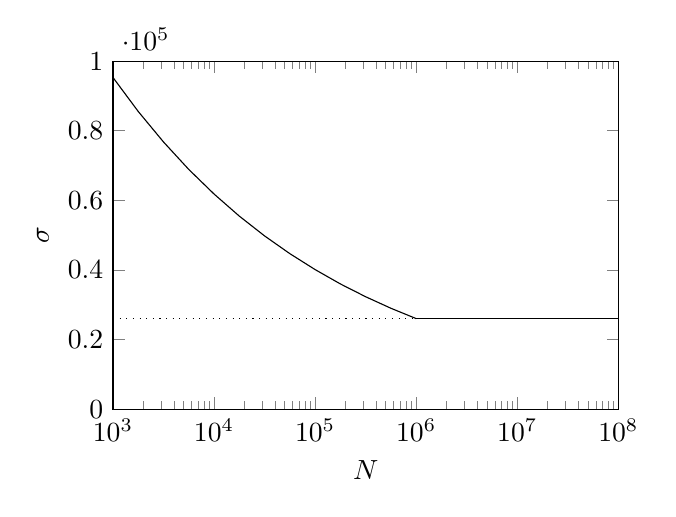
\begin{tikzpicture}
		\begin{semilogxaxis} [
			width = 8cm,
			height = 6cm,
			xlabel = {$N$},
			ylabel = {$\sigma$},
			black,
			xmin = 1000,
			ymin = 0,
			xmax = 100000000,
			ymax = 100000,
			xticklabel style={/pgf/number format/fixed,
                  /pgf/number format/precision=3},
			]
			\addplot+[domain=1:1000000, no marks, black]	
				{349258*x^-0.188};
			\addplot+expression[domain=1000000:100000000, black, no marks]
			{26010};
			\addplot+expression[domain=1000:100000000, black, no marks, dotted]
			{26010};
		\end{semilogxaxis}
	\end{tikzpicture}
\end{wrapfigure}
The aluminum used for this lab does not have a fatigue limit as many ferrous materials do, which can be seen from our trend line not leveling off at some minimum stress amplitude. A material showing some fatigue limit would have a plot resembling Figure 2.
\subsection{Fracture Surface}

For the aluminum used in our tests, the fracture surface was small (<0.2" diameter) and difficult to study conclusively without magnification. Nevertheless, it clearly showed very little evidence of elongation or ductile fracture and no necking. The surface had some small shiny points that could be evidence of crack areas that were worked smooth during the fatigue process. A larger sample from an older test showed clearer characteristics of fatigue fracture. A small shiny area the has radial ridges initiating there, and a rougher surface opposite the shiny area. Figure 3 shows these areas on a ~3/8" diameter aluminum sample.

\vspace{3em}
\begin{figure}[H]
\centering
    \caption{Fatigue Fracture Surface}
		\includegraphics[scale=.15]{cracksurface}
\end{figure}

\pagebreak
\section{Data Analysis}
\begin{multicols}{2}
One complete stress cycle produces a sinusoidal maximum stress amplitude for any point on the surface of our sample at the bending moment. The time for one complete cycle is 0.0171\si{s} derived from our 3500 RPM rotational velocity. Figure 4 shows one stress cycle for first test sample with a bending moment of 30 in$\cdot$lbs.
\begin{figure}[H]
 \caption{Single Stress Cycle}
    \label{tab:graph1}
	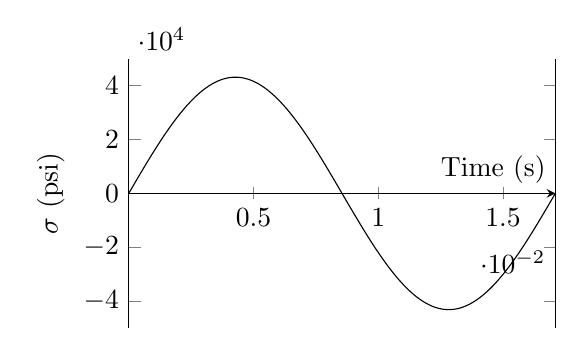
\begin{tikzpicture}
		\begin{axis} [
			width = 7cm,
			height = 5cm,
			xlabel = {Time (s)},
			ylabel = {$\sigma$ (psi)},
			black,
			axis x line=center,
			xmin = 0,
			ymin = -5e4,
			xmax = .0171/(2*pi)*2*pi,
			ymax = 5e4,
			xtick={0.005, 0.01, 0.015},
			]
			\addplot+[samples=500, domain=0:.0171/(2*pi)*2*pi, no marks, black]	
				{43174*sin(deg((2*pi)/0.0171*x))};
		\end{axis}
	\end{tikzpicture}
\end{figure}
\subsection*{Questions}
\begin{enumerate}
\item The fracture did not show any signs of elongation, at least as far as is visible to the naked eye. Compared to a tensile fracture, the fatigue fracture did not neck or appear to tear. There were small lips on the fatigue fracture surface in our tests, but they did not exhibit the characteristic \ang{45} shear surface of ductile fractures and were more rough in texture.

\item Using equation (1), we can find that the stress amplitude corresponding to 100,000 cycles is as follows:
\begin{align*}
\sigma &= 349258*(100000)^{-0.188} \\
\sigma &= 40100 \textrm{ psi}
\end{align*}
For a the factor of safety, we divide $\sigma$ by 1.2 to obtain our maximum allowable stress to survive 100,000 cycles. 
\begin{equation}
\sigma = 33417 \textrm{ psi}
\end{equation}
\item There are many factors which influence the fatigue strength of different materials. As most cracks tend to form at or near the surface of a material, sharp geometric surface discontinuities such as an interior corner or keyway, or rough surface character  produce stress risers than can initiate cracks. To prevent formation of cracks, treatments to increase surface hardness or smooth surface finish are effective at improving fatigue strength. Material composition can also be an important factor for determining fatigue strength. For example, ferrous alloys tend to have a fatigue limit where as most aluminum of any strength or composition will eventually fatigue.
\item
If the specimen were ground prior to the test, the surface would be much smoother which would deter the formation of cracks at the surface. Compared to our S-N curve (Figure 1), we would expect the curve for a surface ground sample to be shifted to the right which would show a larger number of cycles needed to fracture a sample for some known stress amplitude.

\end{enumerate}
\end{multicols}

\section{Conclusion}
Fatigue fracture is a real problem in industry and engineering and accounts for most catastrophic failures in metallic materials. Aerospace structures are especially vulnerable to fatigue since aluminum doesn't have a fatigue limit; in theory, given enough time, all aluminum parts will eventually fail. While we only tested four samples ourselves, in conjunction the extra data from previous experiments we were able to produce a curve fit with a fairly high coefficient of determination, $R^2 = 0.593$. This gives me confidence that our derived expected stress amplitudes to produce failure at various service lives are accurate. It would be interesting to test a ferrous material or other material with a fatigue limit and compare that data to our aluminum samples.
Experimental data recorded during the lab and the lab instructions are attached in the following pages.
\end{document}